\documentclass[11pt, a4paper]{article}
\usepackage[utf8]{inputenc}
\usepackage{graphicx}
\usepackage{float}
\usepackage{pdfpages}
\usepackage{hyperref}
\usepackage{listings}
\usepackage{color}
\usepackage{courier}
\graphicspath{ {./images/} }

\definecolor{dkgreen}{rgb}{0,0.6,0}
\definecolor{gray}{rgb}{0.5,0.5,0.5}
\definecolor{mauve}{rgb}{0.58,0,0.82}

\lstset{%
   breaklines=true,
   basicstyle=\footnotesize\ttfamily,
   language=java,
   columns=fullflexible,
   numbers=left,
   numberstyle=\footnotesize,
}
\hypersetup{
  colorlinks   = true, %Colours links instead of ugly boxes
  urlcolor     = red, %Colour for external hyperlinks
  linkcolor    = black, %Colour of internal links
  citecolor   = blue %Colour of citations
}

\title{assignment}
\author{Matthew Drago }
\date{November 2017}
\begin{document}
\begin{titlepage}
	\centering
	\includegraphics[width=0.15\textwidth]{"uomlogo"}\par\vspace{1cm}
	{\scshape\LARGE University of Malta \par}
	\vspace{1cm}
	{\huge\bfseries Introduction of Software Testing
	\par}
	\vspace{2cm}
	
    \vspace{1.5cm}
    
	{\Large\itshape Matthew Drago\par}
	\par 441198M
	\vfill
	Credit Code: \par
	CPS3230

	\vfill

% Bottom of the page
	{\large 12/12/18\par}
\end{titlepage}
\tableofcontents
\newpage
\section{Dependencies and Structure}
    The project uses Gradle as it's build system and it is written using Java 10, hence make sure these are installed before compiling the project. This project was built and verified working on Arch Linux.
    \subsection{Building The Project and Running Tests}
    Compiling the main sources: 
    \begin{figure}[H]
        \centering
        \begin{verbatim}
            bash gradlew compileJava
        \end{verbatim}
    \end{figure}
    
    Invoking all tests:
    \begin{figure}[H]
        \centering
        \begin{verbatim}
            bash gradlew test
        \end{verbatim}
    \end{figure}

    Should you require more detail on what each method does you can also generate the Java Doc from gradle:
    \begin{figure}[H]
        \centering
        \begin{verbatim}
            bash gradlew test
        \end{verbatim}
    \end{figure}
    The Java Doc should be found under build/docs/javadoc.

    \subsection{Structure}
        \subsubsection{Java Sources}
            The project sources lie under com.cps3230.assignment.payment, which contain two packages gateway and webapp. The Gateway package houses the backend of the project, including the Payment Processor and is where Tasks 1 and 2 are located. The webapp package houses a Spring Boot application with an embedded server. (Required for Task 3)
            \begin{figure}[H]
                \centering
                \begin{tabular} { p{4.5cm} | p{4.5cm} }
                    Package & Description \\
                    \hline
                    gateway.constants & Contains classes representing constant values; \\
                    gateway.enums & Contains enums such as Card Brands and Transaction States; \\
                    gateway.interfaces & Contains interfaces used by the gateway; \\
                    gateway.utils & Contains utility classes; \\
                \end{tabular}
                \caption{A brief description of packages in the Gateway package}
            \end{figure}
        \subsubsection{Test Sources}
            The test sources use the same package structure as mentioned before.
            \begin{figure}[H]
                \centering
                \begin{tabular} { p{4.5cm} | p{4.5cm} }
                    Package & Description \\
                    \hline
                    gateway.adaptors & Contains abstractions for the ModelJUnit testing suite; \\
                    gateway.helpers & Contains helper classes that enhance the Testing suite; \\
                    gateway.models & Contains Models used by the ModelJUnit testing suite; \\
                    gateway.stubs & Contains Stubbed classes; \\
                    webapp.pageobjects & Contains PageObjects that abstract Selenium functions; \\
                    webapp.stepdefs & Contains gherkin definition classes; \\
                    webapp.utils & Contains helper classes; \\
                \end{tabular}
                \caption{A brief description of packages in the Gateway package}
            \end{figure}
\section{Unit Testing Task}
    \subsection{Parameterised Tests}
        This project heavily uses JUnit5's Parameterised Tests to write concise repeatable tests. A Parameterised Test is similar to a normal test but is run with different arguments. Example the test case checkLuhnWorksCorrectlyWithValidCards will run 5 times, each with a different valid card number. The alternative would be to write five different test cases testing exactly the same thing but passing a different value.
        \begin{lstlisting}[caption=A Parameterised Test using a Value Source]
            @ParameterizedTest
            @ValueSource(strings = {"371449635398431", "4230 6885 1339 5737", "3404 769161 31932",
             "4024 0071 5598 4809", "5423 5299 5706 1290"})
            void checkLuhnWorksCorrectlyWithValidCards(String creditCards) {
                Assertions.assertTrue(processor.verifyLuhn(creditCards),
                String.format("Card number %s should be valid", creditCards));
            }  
        \end{lstlisting}
        Arguments can be also passed through an other helper method and using the annotation @MethodSource. Method sources should return a steam of arguments. Example the following snippet tests the processPayment function whilst passing a CcInfo object with a combination of invalid card types and card numbers with invalid prefixes and or lengths.
        \begin{lstlisting}[caption=An example of a method source]
        private static Stream<Arguments> generateCreditCardDetailsWithInvalidCardTypesAndPrefixes() {
            return Stream.of(
                Arguments.of(new CcInfo("Test User", "", "AMERICAN_EXPRESS", "371449635398431", "10/20", "111")),
                Arguments.of(new CcInfo("Test User", "Test address", "amer", "371449635398431", "10/20", "111")),
                Arguments.of(new CcInfo("Test User", "Test address", "VISA", "371449635398431", "10/20", "111")),
                Arguments.of(new CcInfo("Test User", "Test address", "VISA", "5286529599000892", "10/20", "111"))
            );
        }
        \end{lstlisting}
        \begin{lstlisting}[caption=An example of a test case recieving a method source]
            @ParameterizedTest
            @MethodSource("generateCreditCardDetailsWithInvalidCardTypesAndPrefixes")
            void checkProcessPaymentVerifiesCreditCardDetailsWithInvalidCardTypeAndCardNumber(CcInfo card)
                throws ExecutionException, InterruptedException {
                DateIn2018Stub date = new DateIn2018Stub();
                Assertions.assertEquals(1, processor.processPayment(card, 10, date.getTime()));
            }
        \end{lstlisting}
    \subsection{Test Doubles}
        The test suite makes heavy use of test doubles most notably Stubs, Spies and Mocks.
        \subsubsection{Stubs}
            The test suite contains two stubs: DateIn2018Stub and DateIn2021. These stubs return a date in 2018 and 2021 respectively and are used in the Verify Offline method. The class extends from GregorianCalendar and overrides the constructor to explicitly set the date value.
            \begin{lstlisting}[caption=The DateIn2018Stub]
                public class DateIn2018Stub extends GregorianCalendar {
                    public DateIn2018Stub() {
                        set(Calendar.MONTH, 3);
                        set(Calendar.YEAR, 2018);
                    }
                }
            \end{lstlisting}
            The Verify Offline method's signature had to be changed to accept a date to compare to. This way the stub can be injected into the method from the test suite. For convenience the method was overloaded to accept card info and automatically passes today's date. 
            \begin{lstlisting}[caption=The Verify Offline method signature]
                public CardValidationStatuses verifyOfflineEnum(CcInfo cardInfo, Date date) {
                    ...
            \end{lstlisting}
            \begin{lstlisting}[caption=The overloaded Verify Offline method]
                public CardValidationStatuses verifyOfflineEnum(CcInfo cardInfo) {
                    return verifyOfflineEnum(cardInfo, new Date());
                }
            \end{lstlisting}
            \begin{lstlisting}[caption=An example of a test using a stub]
                @ParameterizedTest
                @ValueSource(strings = {"7992739I871o", "79927398712", "79927398719"})
                void checkOfflineVerificationWithInvalidCardNumbers(String cardNumber) {
                  DateIn2018Stub date = new DateIn2018Stub();
                  CcInfo testCreditCardDetails =
                      new CcInfo("Test User", "Test address", "AMERICAN_EXPRESS", cardNumber, "10/20",
                          "111");
                  Assertions.assertEquals(1, processor.verifyOffline(testCreditCardDetails, date.getTime()));
                }
            \end{lstlisting}
            Hadn't stub been used, the test suite would have to be altered every couple of years as cards that wouldn't have been expired would eventually expire, making the tests fail. This stub ensures the tests are repeatable over time.
        \subsection{Spies}
            Spies are extended stubs as the provide the same features as stubs whilst also checking the interactions between the stubbed object. The traditional spies are used to verify interactions between the database and the process payment method. This was used to verify interactions between payment processor and and the Transaction Database. 
            \begin{lstlisting}[caption="Using the database spy in the test suite"]
                @Test
                void verifyTheTransactionDatabaseIsAccessedWhenPaymentAuthorized()
                    throws ExecutionException, InterruptedException {
                  DatabaseSpy databaseSpy = new DatabaseSpy();
                  ...
                  processor.setConnection(databaseSpy);
                  processor.processPayment(testCard, 10, date.getTime());
                  Assertions.assertTrue(databaseSpy.isAccessed(), "Transaction should be accessed");
                } 
            \end{lstlisting}
            \begin{lstlisting}[caption=The database spy impmplemention]
                public class DatabaseSpy implements DatabaseConnection {

                    private Map<Long, Transaction> database;

                    private int requestCount;

                    public DatabaseSpy() {
                        database = new HashMap<>();
                        requestCount = 0;
                    }

                    @Override
                    public boolean saveTransaction(Transaction transaction) {
                        database.put(transaction.getId(), transaction);
                        requestCount++;
                        return true;
                    }

                    @Override
                    public Map<Long, Transaction> getDatabase() {
                        return database;
                    }

                    public int getRequestCount() {
                        return requestCount;
                    }

                    public boolean isAccessed() {
                        return requestCount > 0;
                    }
                }
            \end{lstlisting}
            This project also uses Mockito's spy functionality to verify the interactions between certain objects. This works by mocking the object of interest and then calling the verify method from Mockito. If the method was not called it throws an assertion exception and the test fails.
            \begin{lstlisting}[caption=Using mockito to spy on the bank proxy]
                @Test
                void checkIfBankProxyAuthIsBeingCalledFromProcessPayment()
                    throws ExecutionException, InterruptedException {
                  BankProxy proxy = spy(BankProxy.class);
                  DateIn2018Stub date = new DateIn2018Stub();
                  CcInfo testCard = new CcInfo("Test User", "test address", "AMERICAN_EXPRESS", "371449635398431",
                      "10/20", "111");
                  processor.setBankProxy(proxy);
                  processor.processPayment(testCard, 10, date.getTime());
                  verify(proxy).auth(testCard, 10);
                } 
            \end{lstlisting}
        \subsubsection{Mocks}
            Mock objects combine the benefits of stubs and spies whilst also verify SUT behaviour. They are heavily used in the test suite and are created using mockito. Since the BankProxy class will be provided by the bank, it had to be mocked to verify the payment processor.
            \begin{lstlisting}
                @Test
                void checkProcessPaymentFailsWhenAuthorisationFailsBecauseBankDetailsInvalid()
                    throws ExecutionException, InterruptedException {
                    DateIn2018Stub date = new DateIn2018Stub();
                    BankProxy proxy = mock(BankProxy.class);
                    CcInfo testCard = new CcInfo("Test User", "test address", "AMERICAN_EXPRESS", "371449635398431",
                        "10/20", "111");
                    when(proxy.auth(testCard, 10)).thenReturn((long)-1);
                    processor.setBankProxy(proxy);
                    Assertions.assertEquals(2, processor.processPayment(testCard, 10, date.getTime()));
                }
            \end{lstlisting}
            Mocks where also used to simulate a late response from the database proxy.
            \begin{lstlisting}[caption=Delaying responses from bank proxy]
                when(proxy.capture( 111)).thenAnswer(new Answer<Long>() {
                    @Override
                    public Long answer(InvocationOnMock invocation) throws InterruptedException {
                        Thread.sleep(2000);
                        return (long) 0;
                    }
                });
            \end{lstlisting}
    \subsection{Deviation from the Specification}
        Some changes to the specification where made to increase code quality, and to make the source more testable.
        \subsubsection{Transaction Database}
            A Database connection interface was created in order for the payment processor to accept the database test spy. The payment processor also has a special getter that automatically initializes a transaction database if it's null, thus avoiding any Null Pointer Exceptions. Data sources should extend this interface to integrate with the payment processor.
            \begin{lstlisting}
                public interface DatabaseConnection {
                    boolean saveTransaction(Transaction transaction);
                    Map<Long, Transaction> getDatabase();
                }
            \end{lstlisting}
            For simplicity the transaction database was implemented using a Hash Map. 
            \begin{lstlisting}
                public class TransactionDatabase implements DatabaseConnection {

                    Map<Long, Transaction> database;

                    TransactionDatabase() {
                        database = new HashMap<>();
                    }
                    ...
            \end{lstlisting}
        \subsubsection{CcInfo}
            The CcInfo class holds information related to card details. Some modifications where made to include most of the verification code in the getters and setters of CcInfo. Example an invalid date or card would not be allowed to be set. It also has some helper functions related to card detail verification. This allows each function to be tested individually from the CcInfoTests class.
            \begin{lstlisting}
                public boolean setCardExpiryDate(String cardExpiryDate) {
                    boolean valid = true;
                    SimpleDateFormat simpleDateFormat = new SimpleDateFormat("mm/YY");
                    simpleDateFormat.setLenient(false);
                    try {
                        simpleDateFormat.parse(cardExpiryDate);
                        this.cardExpiryDate = cardExpiryDate.replaceAll("\\s+", "");
                    } catch (ParseException e) {
                        valid = false;
                    }
                    return valid;
                }
            \end{lstlisting}
            \begin{lstlisting}[caption=A helper function that checks the card prefixes]
                protected boolean validatePrefix() {
                    boolean validity = false;
                    if (CardLengths.getCardLengths().get(getCardTypeEnum())
                        .contains(getCardNumber().length()) && CardPrefixes.validPrefixes().get(getCardTypeEnum())
                        .contains(getCardNumberPrefix())) {
                      validity = true;
                    }
                    return validity;
                }
            \end{lstlisting}
        \subsubsection{Payment Processor}
            The specifications for payment processor mentions three methods, namely processPayment, verifyOffline and verifyLuhn. The verify luhn method has not changed from the specification. The verify offlineMethod is simply a wrapper to another method, verifyOfflineEnum which returns an enum representation of the error message. It does not make sense to test some of these overloaded methods as they just call the main verifyOfflineEnum method and pass some default parameters.
            \begin{lstlisting}[caption=Verify offline overloaded methods]
                public int verifyOffline(CcInfo cardInfo) {
                    return verifyOfflineEnum(cardInfo, new Date()).ordinal();
                }

                public int verifyOffline(CcInfo cardInfo, Date date) {
                    return verifyOfflineEnum(cardInfo, date).ordinal();
                }

                // The verify offline method where the main processing is done.
                public CardValidationStatuses verifyOfflineEnum(CcInfo cardInfo, Date date) {
                    CardValidationStatuses cardValidityStatus = CardValidationStatuses.VALID;
                    if (!cardInfo.verifyAllDetailsAreEntered()) {
                        cardValidityStatus = CardValidationStatuses.EMPTY_FIELDS;
                    } else if (!verifyLuhn(cardInfo.getCardNumber())) {
                        cardValidityStatus = CardValidationStatuses.LUHN_FAILURE;
                    } else if (cardInfo.getCardTypeEnum() == CardBrands.INVALID) {
                        cardValidityStatus = CardValidationStatuses.CARD_BRAND_NOT_VALID;
                    } else if (!cardInfo.validatePrefix()) {
                        cardValidityStatus = CardValidationStatuses.PREFIX_NOT_VALID;
                    } else if (cardInfo.validateCardIsNotExpired(date) == CardValidationStatuses.CARD_EXPIRED) {
                        cardValidityStatus = CardValidationStatuses.CARD_EXPIRED;
                    }
                    return cardValidityStatus;
                }
            \end{lstlisting}
            \paragraph{Process Payment} This method's signature was changed drastically. The method executes requests to the payment processor asynchronously thus it accepts an Executor service to which it latches asynchronous methods to. Once a transaction gets authorized it is saved on to the database and it's status is saved as \emph{CAPTURE}. Every time the processor is called it calls another asynchronous method that tries to capture all transactions in the \emph{CAPTURE} state. However there is a processPayment method whose signature matches with the specification. The process payment relies on two wrapper functions, one that authorizes a transaction and an other that captures a transaction by calling their respective methods in the bank proxy.
            \begin{lstlisting}[caption=A wrapper function that calls the bankporxy asynchronously and returns a Transaction if valid]
                private Callable<Transaction> authoriseCallable(CcInfo cardInfo, long amount) {
                    return () -> {
                      Transaction transaction = null;
                      long transactionId = getBankProxy().auth(cardInfo, amount);
                      if (transactionId > 0) {
                        transaction = new Transaction(transactionId, cardInfo, amount, TransactionStates.CAPTURE);
                      } else {
                        LOGGER.info("Bank error - bank returned status code {} - payment rejected", transactionId);
                      }
                      return transaction;
                    };
                }
            \end{lstlisting}
            \begin{lstlisting}[caption=A wrapper method that calls the bank proxy asynchronously and ]
                Callable<Transaction> captureCallable(Transaction transaction) {
                    return () -> {
                        int status = getBankProxy().capture(transaction.getId());
                        switch (status) {
                            case 0: {
                                transaction.setState(TransactionStates.CAPTURED.toString());
                                break;
                            }
                            case -1: {
                                transaction.setState(TransactionStates.BANK_DETAILS_INVALID.toString());
                                break;
                            }
                            case -2: {
                                transaction.setState(TransactionStates.CAPTURED.toString());
                                break;
                            }
                            case -3: {
                                transaction.setState(TransactionStates.VOID.toString());
                                break;
                            }
                            default: {
                                transaction.setState(TransactionStates.AUTHORIZED.toString());
                            }
                        }
                        return transaction;
                    };
                }
            \end{lstlisting}
        \subsubsection{Update Database Transactions} 
            Since \emph{AUTHORIZED} transactions get saved in the database a function was created that periodically gets all transactions with an \emph{AUTHORIZED} state and tries to capture them. This method can then be called with a scheduled executor and run periodically.

            \begin{lstlisting}
                Callable<Void> updateTransactions(ExecutorService executorService, CountDownLatch latch) {
                    return () -> {
                      Map<Long, Transaction> authorizedTransactions = getConnection().getDatabase()
                          .entrySet().stream()
                          .filter(x -> x.getValue().getState().equals(TransactionStates.AUTHORIZED.toString()))
                          .collect(
                              Collectors.toMap(Map.Entry::getKey, Map.Entry::getValue));
                      authorizedTransactions.forEach((transId, transaction) -> {
                        try {
                          Future<Transaction> captureFuture = executorService.submit(captureCallable(transaction));
                          Transaction capturedTransaction = captureFuture.get();
                          getConnection().saveTransaction(capturedTransaction);
                        } catch (InterruptedException | ExecutionException e) {
                          LOGGER.error(e.getLocalizedMessage());
                        }
                      });
                      latch.countDown();
                      return null;
                    };
                }
            \end{lstlisting}
    \subsection{Coverage}
        \begin{figure}[H]
            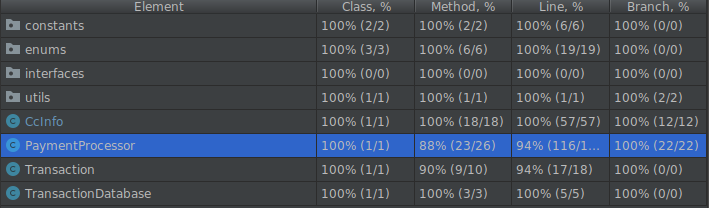
\includegraphics[width=\textwidth]{coverage}
            \caption{The overall test coverage}
        \end{figure}
        Because of the overloaded methods 100\% line coverage could not be achieved, however 95\% coverage in the PaymentProcessor is acceptable. It should be noted that the test suite has 100\% branch coverage. This means every decision in the code base was hit from the test suite at least once. There was one getter method in the Transaction class that only does simple assignment which was not tested. In general simple getters and setters were not tested individually but were called from other methods in the source. Getters and setters were only tested if they carried out logic. All other classes feature 100\% line, class, method and branch coverage.
\newpage
\section{Model Testing}
    The model tests can be run by running the TransactionModelTest class and are run automatically when you run the test task from gradle. There are three tests the first being runModelTestsWithGreedyTester which executes the model test using a greedy tester. The second test is a unit test that uses an all round tester and the third launches an all round tester. During experimentation it was discovered that the greedy tester works best, hence it's the only test that runs by default whilst the others are ignored.
    The greedy tester achieves 100\% action, state and transition coverage with a test length of 150.
    \begin{lstlisting}
        @Test
        void runModelTestsWithGreedyTester() {
            TransactionModel model = new TransactionModel();
            Tester tester = new GreedyTester(model);
            tester.buildGraph();
            tester.addListener(new VerboseListener());
            tester.addListener(new StopOnFailureListener());
            tester.addCoverageMetric(new TransitionCoverage());
            tester.addCoverageMetric(new StateCoverage());
            tester.addCoverageMetric(new ActionCoverage());
            tester.generate(100);
            tester.printCoverage();
        }
    \end{lstlisting}
    The Transaction model also makes use of a PaymentProcessorAdaptor that abstracts some of the detail in calling the payment processor and avoid cluttering up the model.
    \begin{lstlisting}[caption=A snippet showing how some of the abstraction is done]
        public Transaction tryToRecaptureBecauseBankError() throws ExecutionException, InterruptedException {
            CcInfo testCreditCardDetails = new CcInfo("Test User", "Test address", "AMERICAN_EXPRESS", "371449635398431", "10/20", "111");
            BankProxy mockProxy = mock(BankProxy.class);
            when(mockProxy.capture((long) 111)).thenReturn(-4);
            processor.setBankProxy(mockProxy);
            Transaction transaction = new Transaction((long) 111, testCreditCardDetails, 10, "AUTHORIZED");
            return processor.capture(transaction);
        }
    \end{lstlisting}
    The following page includes a diagram of the model.
    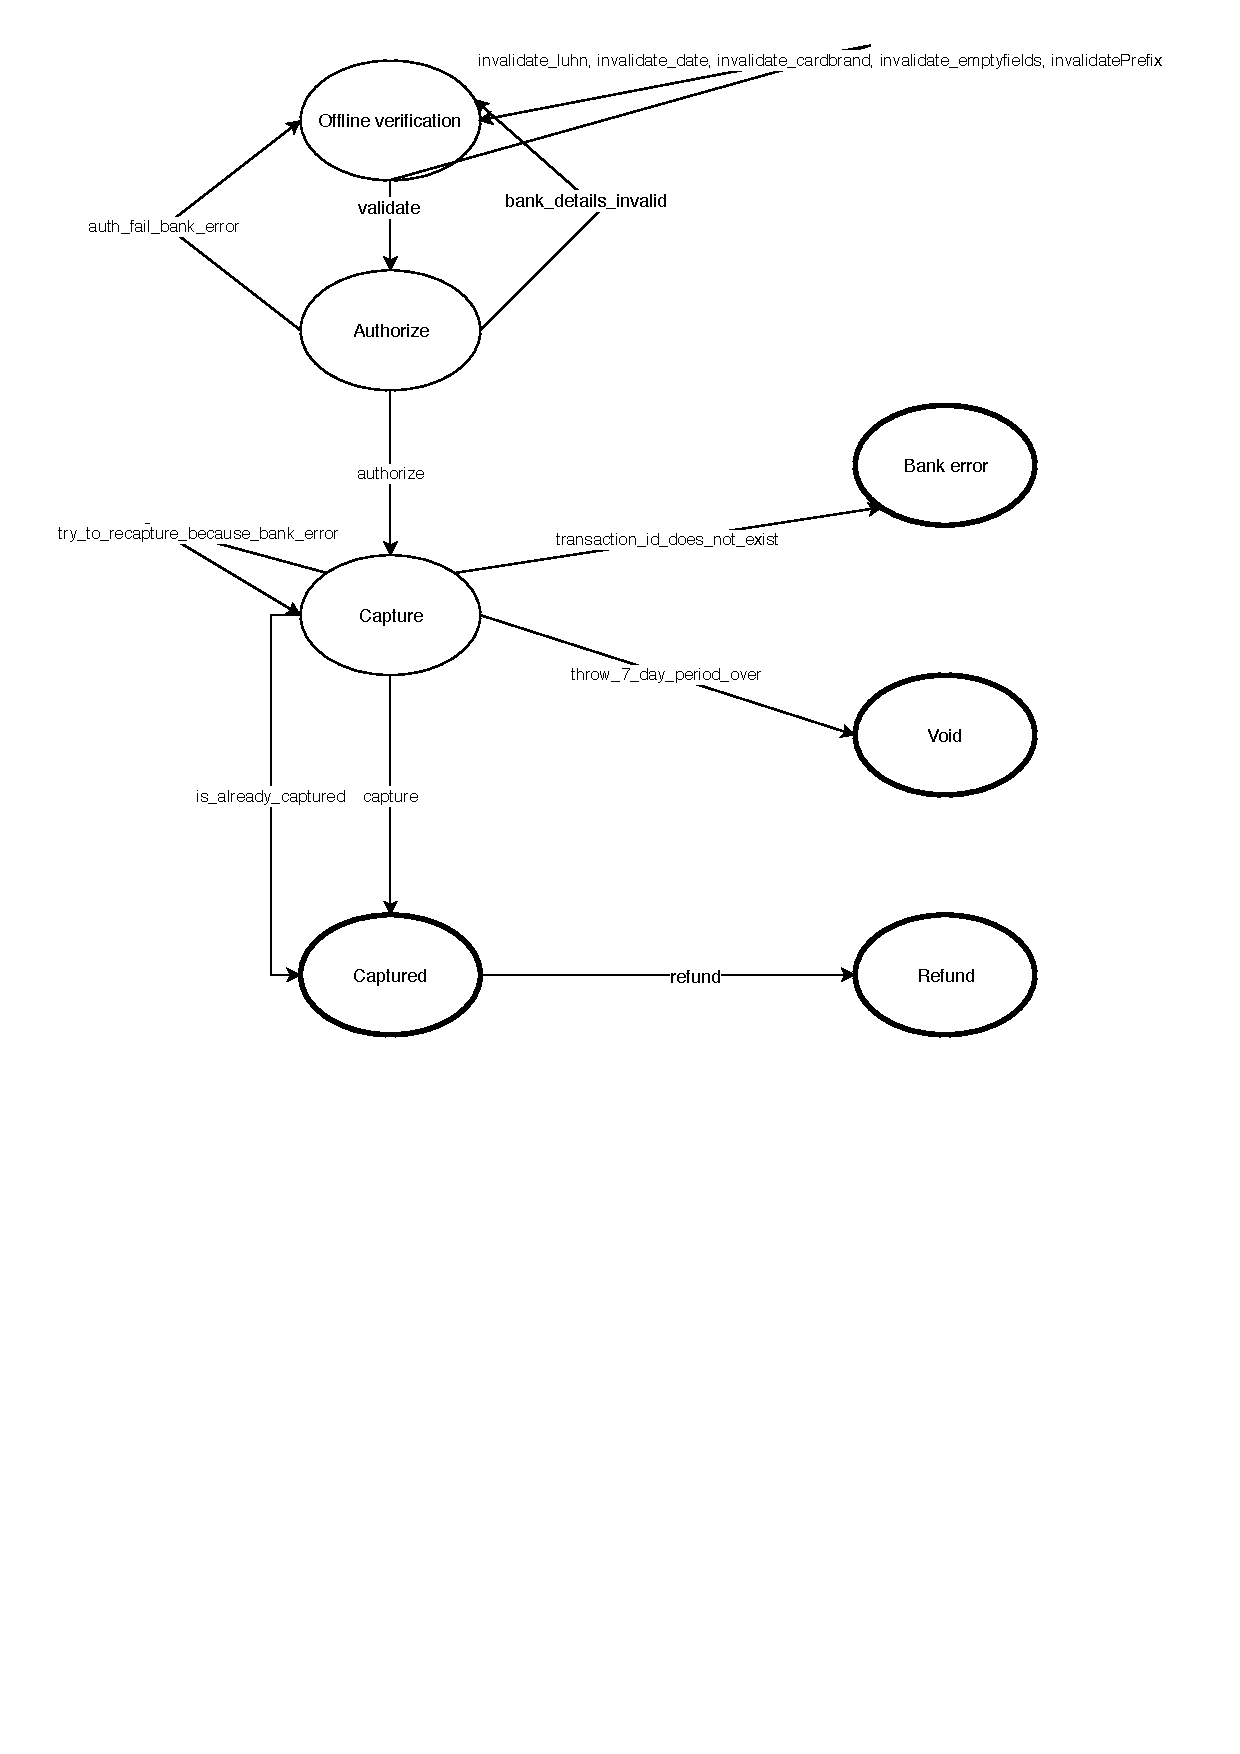
\includepdf{model.pdf}
\section{Cucumber and Automated Web Testing}
    The web interface was implemented using Spring Boot and can be found in the com.cps3230.assignment.payment.webapp package. The cucumber feature files are located under test/resources/features. Spring Boot was used as the web framework as it bundles it's own server thus making it easy to get a web service up and running.
    Running the server from the command line without mocks:
    \begin{verbatim}
        bash gradlew bootRun
    \end{verbatim}
    \emph{Note} Due to an internal tomcat bug, web tests might fail because an exception is thrown during server shutdown despite the cumber tests passing.

    \paragraph{Running the Tests}
    \begin{lstlisting}[language=bash]
        bash gradlew test --tests "com.cps3230.assignment.payment.webapp.PaymentProcessorWebTests"
    \end{lstlisting}
    
    \paragraph{} During the test task a server is run with a mocked Bank Proxy. 
    \subsection{Browser Driver}
        The Browser Driver is a singleton class that returns a Web driver instance.
        \begin{lstlisting}[caption=Getting a Web Driver Instance]
            public synchronized static WebDriver getCurrentDriver() {
                if (mDriver == null) {
                    try {
                        System.setProperty("webdriver.chrome.driver", "/home/drago/chromedriver");
                        mDriver = new ChromeDriver();
                    } finally {
                        Runtime.getRuntime().addShutdownHook(
                            new Thread(new BrowserCleanup()));
                    }
                }
                return mDriver;
            }
        \end{lstlisting}
    \subsection{Page objects}
        Page objects abstract selenium calls that interact with the webpage. The project implemented the Page Object pattern in the Payment Webapp Page Object class. It contains functions for entering details in the form, submitting the form getting entered information etc\dots
        \begin{lstlisting}[caption=A method in the Payment Webapp Page Object that facilitates form entry]
            public void enterDetails(EntryObject entry) {
                driver.findElement(By.name("customerName")).sendKeys(entry.getCustomerName());
                driver.findElement(By.name("customerAddress")).sendKeys(entry.getCustomerAddress());
                final Select selectBox = new Select(driver.findElement(By.name("cardType")));
                selectBox.selectByValue(entry.getCardType());
                driver.findElement(By.name("cardNumber")).sendKeys(entry.getCardNumber());
                driver.findElement(By.name("cardExpiryDate")).sendKeys(entry.getCardExpiryDate());
                driver.findElement(By.name("cardCvv")).sendKeys(entry.getCardCvv());
                driver.findElement(By.name("amount")).sendKeys(entry.getAmount());
              }
        \end{lstlisting}
    \subsection{Cucumber}
        To be able to inject a mocked Bank proxy the cucumber tests are launched through a Spring Boot Test. This allows the controller to be wired up. The class PaymentProcessorWebTests launches the cucumber tests.
        \begin{lstlisting}[caption=The unit test that launches the cucumber tests]
            @Test
            public void runCucumberTests() {
                cucumber.api.cli.Main.main(new String[]{
                    "--glue",
                    "com.cps3230.assignment.webapp.stepdefs",
                    "src/test/resources/features/webapp_features.feature"
                });
            }
        \end{lstlisting}
        The WebappDefs class defines all of the step definitions that are required by the feature files.
        \begin{lstlisting}[caption=A step definition using a cucumber expressions]
            @When("I submit a form with all data but {string} is invalid")
            public void submitAFormWithAllDataButIsInvalid(String date) throws InterruptedException {
              EntryObject entry = new EntryObject("Test User", "Test Address", "AMERICAN_EXPRESS", "371449635398431", date, "111", "10");
              webappPageObject.enterDetails(entry);
              webappPageObject.submitDetails();
            }
        \end{lstlisting}
% \newpage
% \bibliographystyle{plain} 
% \bibliography{references}

\end{document}
